\documentclass{../../../tp}


\title{Practical Session 7: \prolog}
\author{}

\begin{document}
	
\maketitle

\section{Caching}

Fibo assert
	
\section{is}	

We have seen that arithmetic expressions are not necessarily evaluated directly. This is where the \prologcode{is} predicate comes into play. 
The predicate

\begin{lstlisting}[language=prolog]
	Number is Expr
\end{lstlisting} 

is \prologcode{true} whenever \prologcode{Expr} evaluates to \prologcode{Number}. 


\begin{instruction}
	Write a \prologcode{power(X, N, Z)} procedure to compute $Z = X^N$. 
	
\end{instruction}

\todo[inline]{Exemple utilisation de power (var, const, const)  (const, var, const)  etc...
	+     X is 3 + Y   error
	}

\section{Cuts}

Backtracking is at the core of the logic engine, and sometimes it could be useful to have some control on how \prolog explores the search tree. The cut operator is one way of doing this. This predicate is written \prologcode{!} and is always true. This operator forces \prolog to commit all choices made before the cut and not consider other choices for the already bound variables. It divides the body of a rule in two parts: once the cut is passed (because all previous terms have found possible solutions), no more backtracking will be done for the first part. Backtracking in the second part is performed as usual.

\begin{instruction}
	\begin{enumerate}
		\item Implement a \prologcode{f(X,Result)} predicate to implement the following function (without using cuts):
		
		$$ f(x) = \begin{cases} 
		0 & \textrm{if $x < 3$}  \\ 
		2 & \textrm{if $3 \leq x < 6$} \\
		4 & \textrm{if $6 \leq x$} 
		\end{cases} $$
		
		Why is your implementation not optimal in terms of backtracking? 
		
		\item Consider the following implementation: 
		
		\begin{lstlisting}[language=prolog]
		f(X,0) :- X<3, !.
		f(X,2) :- 3≤X, X<6, !.
		f(X,4) :- 6≤X,!.
		\end{lstlisting}
		
		Why is this implementation equivalent to the first one, but more efficient? 
	\end{enumerate}
\end{instruction}

You might notice that this implementation could make use of the order of the rules, to be rewritten as:

\begin{lstlisting}[language=prolog]
	f2(X,0) :- X<3, !.
	f2(X,2) :- X<6, !.
	f2(X,4).
\end{lstlisting}

This is almost equivalent to the previous notation (can you tell the difference? Think for instance about what a query like \prologcode{f2(1,2)} would return). However, it violates a good practice in \prolog: each rule should be able to be taken and understood by itself. For instance, if you take the last expression of the first version :
\begin{lstlisting}[language=prolog]
	f(X,4) :- 6≤X,!.
\end{lstlisting}

This can be read: ``$f(X,4)$ is true whenever $X$ is greater or equal than 6'', or in other words ``$f(X) = 4$ if $X \geq 6$'' which is coherent with the mathematical definition of $f$. However, in the second version: 
\begin{lstlisting}[language=prolog]
	f2(X,4).
\end{lstlisting}

we can read ``$f2(X,4)$ is true'' which is incorrect, based on the mathematical definition of $f$, unless you know that there are other, previous rules, taking care all of cases where $X < 6$. This expression cannot be taken separately of the others and still make proper sense. We say that $f2$ uses a \emph{red cut}, whereas the first version which respects the good practice is said to use a \emph{green cut}.

Green cuts can be used to prevent \prolog from exploring useless paths. They only affect efficiency, but not the meaning of the program. Red cuts change the meaning of the program, and make it harder to read a program. They should be used more cautiously.

\begin{instruction}
	
	\begin{enumerate}
		\item Write a  \prologcode{merge(List1, List2, Result)} predicate, which merges two sorted lists into a new sorted list, without the use of a cut.
		\item Use a green cut to exploit the mutually exclusive nature of the tests. Watch where you place the cuts!
		\item Rewrite the predicate even more efficient by making use of a red cut.
		
	\end{enumerate}
	
	
	
\end{instruction}

\section{Meta-interpreter}

In \prolog, it is easy to write expressions which manipulate other expressions in the language. For instance, consider the following meta-interpreter :

\begin{lstlisting}[language=prolog]
solve(true) :-!.
solve(not A) :- not(solve(A)).
solve((A, B)) :-!, solve(A), solve(B).
solve(A) :- clause(A, B), solve(B).
\end{lstlisting}

\prologcode{solve} takes as argument a goal and processes it following the semantics of \prolog. 

\begin{instruction}
	Can you understand how this works? What does the \prologcode{clause/2} predicate do? If you have trouble understanding what  \prologcode{clause} does, try for instance to look at what \prologcode{clause(power(0,0,1), Body)} gives for possibles values of \prologcode{Body}. \\
	
	Try to modify the \prologcode{solve/1} predicate into a \prologcode{solve/2} predicate, where the second parameter is used to return a \emph{proof tree} for the goal given in first parameter. For instance:
	
	\begin{lstlisting}[language=prolog]
	?- solve(grandparent(george,alexandra), Proof).
	Proof = (grandparent(george, alexandra) :- 
		    (parent(george, maria) :- 
		        (father(george, maria) :- true)),
		    (parent(maria, alexandra) :- 
		        (mother(maria, alexandra) :- true)));
	\end{lstlisting}
\end{instruction}

\todo{warning: limited (operators not supported)}

\todo{Meta-interpreteurs plus complexes -> simply logical}

\section{Eight Queens}

The eight queens puzzle is a problem where, given a standard 8x8 chessboard, you have to place 8 queens such that no queen can attack each other. In case you do not know the rules of chess, this means no two queens can be on the same row, or the same column, or the same diagonal on the board. 

\begin{figure*}[h]
	\centering
	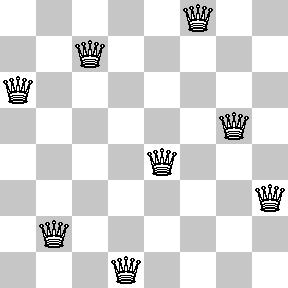
\includegraphics[scale=0.5]{8queens}
	\captionsetup{labelformat=empty}
	\caption{A possible solution for the 8-queens puzzle}
\end{figure*}

Your task is to solve this problem in \prolog.

\begin{instruction}
	\begin{enumerate}
		\item Start by defining a way to model the problem.
		\item Then, implement a \prologcode{safe} predicate which verifies wheter a particular configuration of queens on the board is safe (no queen can attack another). Use an \prologcode{attack} predicate which checks whether one particular queen attacks the others.
		\item Finally, the puzzle can be solved by simply checking all possible configurations of the board
	\end{enumerate}
	
	As a side-exercise, for the most motivated students: can you improve the performance of this implementation? Specifically, we could try to avoid exploring all possible configurations and check the safety of a queen directly when is it placed.
\end{instruction}

\end{document}